\documentclass[letterpaper,12pt]{article}
\usepackage{fancyhdr}
\usepackage{amsmath}
\usepackage{amssymb}
\usepackage{bm}
\usepackage{numprint}
\usepackage[margin=1in]{geometry}
\usepackage{graphicx}
% Random packages from
% http://tex.stackexchange.com/questions/50070/landscape-figure-in-latex
% Necessary for sideways pictures
\usepackage{wrapfig}
\usepackage{lscape}
\usepackage{rotating}
\usepackage{epstopdf}
\usepackage{tablefootnote}
% for word wrap verbatim
\usepackage{listings}
\lstset{
   breaklines=true,
   basicstyle=\ttfamily}
% \pagestyle{fancy}
% \lhead{Jesse Mu}
% \rhead{CSCI339 Term Project}
% One more .. since we're in the abbreviated subdir
\graphicspath{ {../../figures/abbreviated/} {../../figures/} }



\begin{document}

\title{Cluster Analysis: Identifying Parkinson's Disease Subtypes}
\author{Jesse Mu}
\maketitle

\section{Preprocessing}

\subsection{Dataset Description}
951 subjects, 145 metrics, collected 15-4-2012 from Pablo Martinez Mart\'in. Only
19 features used for clustering and/or interpretation.  50 subjects with
missing values of the features to be used in clustering (brought down to 901).
It was decided to not impute the data.

\subsection{Selected Features}

Combination of non-motor scale (NMS) symptoms and standard motor symptoms.
PIGD was deleted after 2015-07-16 meeting.

\begin{table}[h]
  \centering
  \begin{tabular}{l|l|l}
    Name & Type & Description \\
    \hline
    nms\_d1 & byte & cardiovascular \\
    nms\_d2 & byte & sleep/fatigue \\
    nms\_d3 & byte & mood/cognition \\
    nms\_d4 & byte & percep/hallucinations \\
    nms\_d5 & byte & attention/memory \\
    nms\_d6 & byte & gastrointestinal \\
    nms\_d7 & byte & urinary \\
    nms\_d8 & byte & sexual function \\
    nms\_d9 & byte & miscellaneous \\
    tremor & float & tremor \\
    bradykin & float & bradykinesia\tablefootnote{Impaired ability to
    adjust the body's position.} \\
    rigidity & float & rigidity \\
    axial & float & axial\tablefootnote{Issues affecting the middle of
    the body.} \\
  \end{tabular}
  \caption{Selected Features and Details}
  \label{tab:selected-features}
\end{table}

\begin{table}[h]
  \centering
  \begin{tabular}{l|l|l|l}
  Name  &       $\mu$ & $\sigma$ & min-max \\
         \hline
nms\_d1&   1.73&  3.35&   0-24 \\
nms\_d2&   8.75&  8.70&   0-48 \\
nms\_d3&   8.68& 11.55&   0-60 \\
nms\_d4&   1.64&  3.86&   0-33 \\
nms\_d5&   5.42&  7.43&   0-36 \\
nms\_d6&   5.53&  6.79&   0-36 \\
nms\_d7&   8.08&  8.94&   0-36 \\
nms\_d8&   3.52&  5.97&   0-24 \\
nms\_d9&   7.13&  7.79&   0-48 \\
tremor&   2.59&  2.58&   0-12 \\
bradykin& 2.40&  1.41&   0-6 \\
rigidity& 2.24&  1.36&   0-6 \\
axial&    3.25&  2.68&   0-12 \\
  \end{tabular}
  \caption{Descriptive Statistics}
  \label{tab:descriptive-statistics}
\end{table}

\section{Clustering}

$k$-means clustering with $k = 4$ was tried. Statistics for determining the
optimal number of clusters were used, but were inconclusive: results in
Figure~\ref{tab:numclus}. This probably indicates that the data is not very
well clustered. $k = 2, 3$ provided models that were too simplistic. $k = 5$
did not provide any new information, but rather just fragmented existing
groups.
\begin{table}[h]
  \centering
  \begin{tabular}{l|l}
    Criterion & Optimal $k$ \\
    \hline
    Minimum ASW & 2 \\
    BIC & 18 \\
    SSE Scree Plot & Inconclusive \\
    Gap Statistic & 4, 13? \\
    Affinity Propagation\tablefootnote{$\lambda = 0.98$, q = 0, maxits = 1000,
    convits = 100} & 8 \\


  \end{tabular}
  \caption{Results of various techniques for determining $k$}
  \label{tab:numclus}
\end{table}

\subsection{Decision tree}
% \begin{table}[h]
  % \centering
  % \begin{tabular}{l|l|l|l|l|l}
    % $k$ & CP\tablefootnote{Complexity Parameter} & CV Xerror\tablefootnote{10-fold cross
    % validation} & Root Feature &
    % Root Error & Figure \\
    % \hline
    % 4 & 0.0100 & 0.255 & pigd $<$ 2.5 & 0.563 & Figure~\ref{fig:kmeans-dtree-4} \\
  % \end{tabular}
  % \caption{$k$-kmeans decision trees statistics}
  % \label{tab:k-means-dtrees}
% \end{table}

Decision tree for $k = 4$ created via recursive partitioning is available in
Figure~\ref{fig:kmeans-dtree-4}. More discussion about the decision tree is
located in Section~\ref{feature-importance}.

\begin{figure}[h]
  \centering
  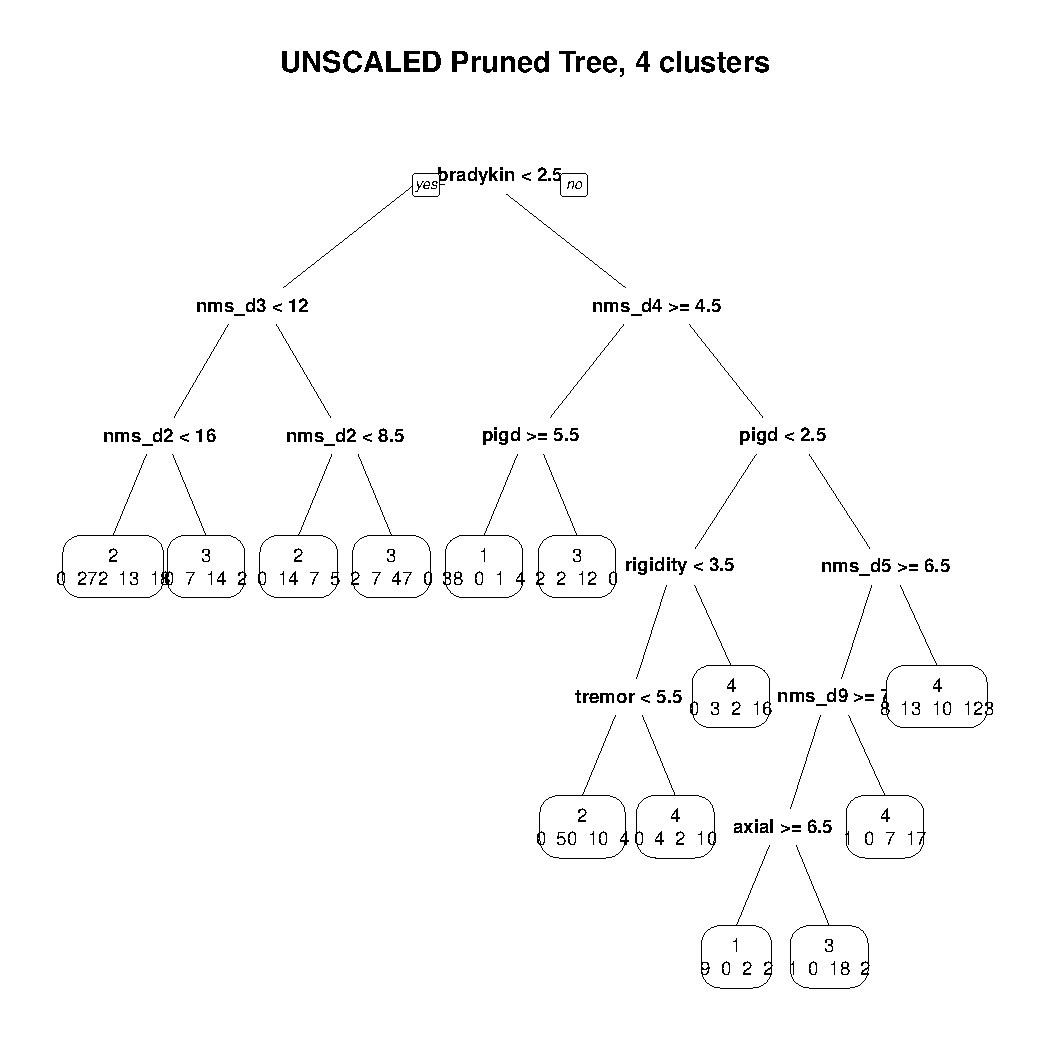
\includegraphics[width=\linewidth]{dtree-kmeans-pruned-unscaled-4.pdf}
  \caption{Decision Tree from $k$-means clustering, 4 clusters}
  \label{fig:kmeans-dtree-4}
\end{figure}

\subsection{Interpretation of Clusters}

\subsubsection{Cluster summaries}

Available in Figure~\ref{fig:kmeans-summaries-4}. Error bar is standard error.

\begin{figure}[h]
  \centering
  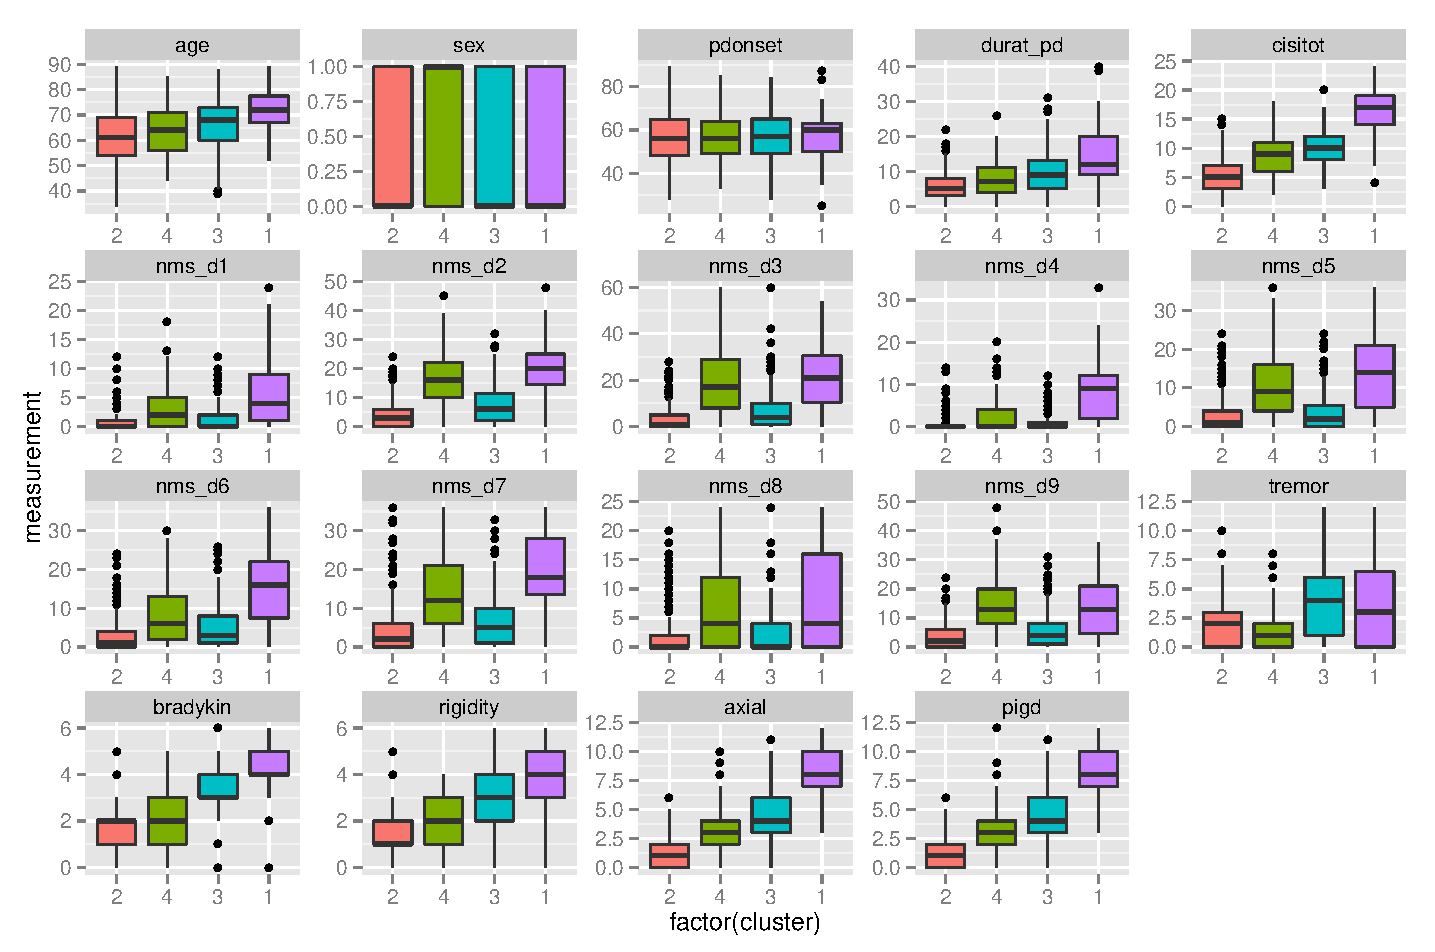
\includegraphics[width=\linewidth]{kmeans-summaries-4.pdf}
  \caption{Cluster Summaries, $k = 4$}
  \label{fig:kmeans-summaries-4}
\end{figure}

\subsubsection{Interpretation}
$k$-means clustering ($k = 4$) found four clusters. They are numbered (somewhat
confusingly) according to the automatically assigned numbers of the cluster
analysis, and not by any intuitive pattern. With a brief description, they are:

\begin{itemize}
  \item[4.] $(n = 406)$ Mildly affected in all domains.
  \item[1.] $(n = 189)$ Severely affected in nonmotor domains; mildly
    affected in motor domains.
  \item[3.] $(n = 221)$ Severely affected in motor domains; mildly
    affected in nonmotor domains.
  \item[2.] $(n = 88)$ Severely affected in all domains.
\end{itemize}

These cluster results are identical to the four clusters found in van Rooden et
al \cite{vanrooden10}, which was done with a separate dataset using a different
modeling method (expectation-maximization), supporting these subtype
classifications. Unlike van Rooden, mean disease durations differences do exist
between subtypes 4 (mild) and 2 (severe), likely due to further development of
the disease, although the differences between 1 and 3 (nonmotor/motor
predominated) subtypes are insignificant, suggesting different developmental
paths of the disease.

\subsubsection{Statistical Significance Tests, $k = 4$}
Using one-way ANOVA for multiple means, we reject the null
hypothesis that the means are the same with $p < 0.05$ for every variable
\emph{except} pdonset.

Post-hoc analysis using Tukey's HSD to examine statistically significant
differences between individual means is available in Table~\ref{tab:tukeyhsd}.
Only statistically insignificant relations are provided; all other relations
are significant with $p < 0.05$.

\begin{table}[h]
  \centering
  \begin{tabular}{l|l|l}
  Variable & Cluster Relation & $p$ \\
  \hline
  age & 3-1 & 0.724 \\
      & 4-1 & 0.428 \\
  \hline
  sex & 2-1 & 0.849 \\
      & 4-1 & 0.092 \\
      & 3-2 & 0.161 \\
      & 4-2 & 0.827 \\
      & 4-3 & 0.216 \\
  \hline
  pdonset & 2-1 & 0.147 \\
          & 3-1 & 0.370 \\
          & 4-1 & 0.859 \\
          & 3-2 & 0.803 \\
          & 4-2 & 0.305 \\
          & 4-3 & 0.700 \\
  \hline
  durat\_pd & 3-1 & 0.562 \\
  \hline
  cisitot & 3-1 & 0.523 \\
  \hline
  nms\_d1 & 4-3 & 0.333 \\
  \hline
  nms\_d4 & 4-3 & 0.557 \\
  \hline
  nms\_d5 & 4-3 & 0.856 \\
  \hline
  nms\_d8 & 4-3 & 0.122 \\
  \hline
  nms\_d9 & 2-1 & 0.730 \\
         & 4-3 & 0.074 \\
  \hline
  tremor & 4-1 & 0.360 \\
  \end{tabular}
  \caption{Tukey's HSD Insignificant Differences}
  \label{tab:tukeyhsd}
\end{table}

\subsubsection{Feature importance}
\label{feature-importance}

Features ranked by information gain with respect to cluster are available in
Table~\ref{tab:info_gain}. Also, in the 4-cluster decision tree in
Figure~\ref{fig:kmeans-dtree-4}, features are ranked implicitly by importance
in determining clusters. We see, quite naturally, that standard measures of
motor symptoms rank very highly (1, 2, 4, 5) in information gain \emph{except}
termor (12). Similarly, bradykinesia (1) is used as the root node of the
4-cluster decision tree, although other motor symptoms are used further down
the tree, since immediately successive motor symptom decision nodes would, due
to their determination of clusters, be redundant.

The most informative nonmotor
symptoms are nms\_d2 (sleep/fatigue) at 2, along with nms\_d3
(mood/cognition). As discussed later in Section~\ref{sub:ova} these features
become critical in one-versus-all decision trees for distinguishing various
subtypes. The importance of these nonmotor symptoms confirms the longitudinal
study by Fereshtehnejad et al. \cite{fereshtehnejad15} who cites a 3-cluster PD
subtype identification based primarily on nonmotor symptoms including cognitive
impairment, rapid eye movement sleep disorder (RBD), anxiety, and depression,
conditions that align closely with nms\_d2 and nms\_d3 as tested in this
dataset. More analysis needs to be done on whether there are parallels between
Fereshtehnejad's 3-cluster longitudinal study and the clusters found in both
this investigation and van Rooden.

Interestingly, demographic information, including durat\_pd, age, sex, and
pdonset, plays almost no role in the determination of these clusters. That the
time of onset of PD or sex nulls important, clinically-relevant questions about
the demographic sources of these different subtypes.

\begin{table}[h]
  \centering
  \begin{tabular}{l|l|l}
    rank & variable & information gain \\
    \hline
    1 & bradykin      & 0.31574672 \\
    2 & rigidity      & 0.29560018 \\
    3 & nms\_d2      & 0.24218407 \\
    4 & cisitot      & 0.22920103 \\
    5 & axial      & 0.22780750 \\
    6 & nms\_d3      & 0.20480570 \\
    7 & nms\_d9      & 0.15782743 \\
    8 & nms\_d7      & 0.15290569 \\
    9 & nms\_d5      & 0.14454931 \\
    10 & nms\_d6      & 0.14025139 \\
    11 & nms\_d1      & 0.13212756 \\
    12 & tremor      & 0.10937168 \\
    13 & nms\_d4      & 0.10710526 \\
    14 & nms\_d8      & 0.10005480 \\
    15 & durat\_pd      & 0.02876190 \\
    16 & age      & 0.02346158 \\
    17 & sex      & 0.00000000 \\
    18 & pdonset      & 0.00000000 \\
  \end{tabular}
  \caption{Features ranked by information gain}
  \label{tab:info_gain}
\end{table}

\subsubsection{Correlation Plots}

The interplay between specific symptoms in each of the four clusters was
examined in Figure~\ref{fig:corrplots}, but nothing too interesting was found. There is, perhaps somewhat
interestingly, a somewhat higher correlation between bradykinesia, rigidity,
and nms\_d6 (gastrointestinal), but it was not judged to be significant.

\begin{figure}[h]
  \centering
  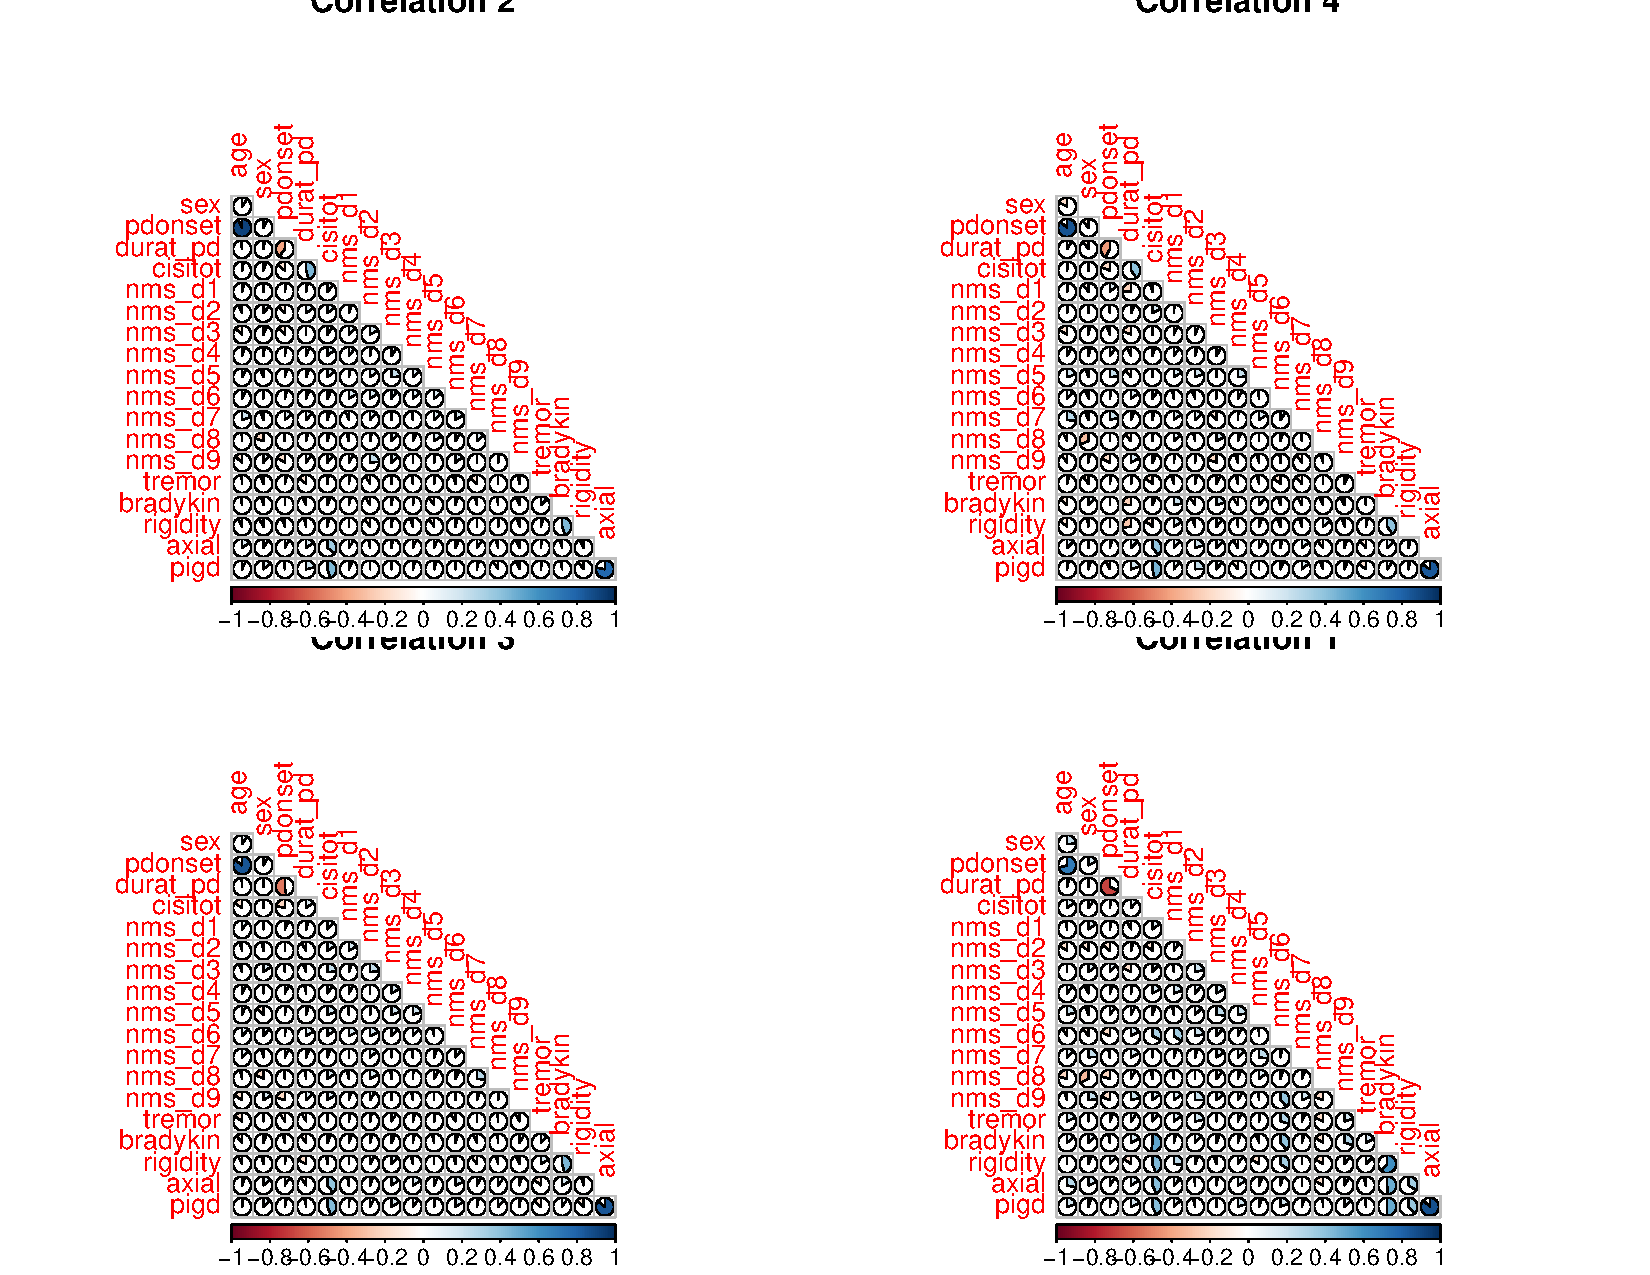
\includegraphics[width=\linewidth]{corrplots.pdf}
  \caption{Correlation plots}
  \label{fig:corrplots}
\end{figure}

\section{Nonmotor-predominant subtype analysis}
\subsection{$k$-means sub-subdivision on Cluster 1}

In an attempt to understand further the properties of the nonmotor-dominated
subtypes, $k$-means analysis was run again on specifically this subtype to
examine any possible patterns.

 The same $k$-determining tests were run on subtype 1 and are displayed
in Table~\ref{tab:numclus-nms}.

\begin{table}[h]
  \centering
  \begin{tabular}{l|l}
    Criterion & Optimal $k$ \\
    \hline
    Minimum ASW & 2 \\
    BIC & 1 (?) \\
    SSE Scree Plot & Inconclusive \\
    Gap Statistic & 3 \\
    Affinity Propagation\tablefootnote{$\lambda = 0.98$, q = 0, maxits = 1000,
    convits = 100} & 5 \\
  \end{tabular}
  \caption{Results of various techniques for determining $k$, applied to
  subtype 1}
  \label{tab:numclus-nms}
\end{table}

Boxplots for $k$-means run for $k = 2, 3, 4$ can
be seen in Figures~\ref{fig:c1-summaries-2},~\ref{fig:c1-summaries-3},
and~\ref{fig:c1-summaries-4}.

\subsection{Interpretation}
\label{sub:nms-interp}

An interesting set of subtleties occurs when $k = 2$ and 3. When $k = 2$, the
two groups
are generally somewhat similar, except nms\_d2 and nms\_d3 move in opposite
directions, i.e.\ sub-subtype 2 generally has higher nms\_d2 scores but lower
nms\_d3 scores. In addition, sub-subtype 2 has higher axial scores. This
difference can be once again observed in $k = 3$, where subtype 3 is shown to
have higher nms\_d2 scores, lower nms\_d3 scores, and higher axial scores. This
may indicate a trend in nonmotor-dominated PD for nms\_d2 and nms\_d3 to live
on opposite ends of a spectrum, i.e.\ patients especially severe in one may not
be as severe in the other. This difference can also been seen in
Section~\ref{sub:ova}, when OVA decision trees are discussed for the the
nonmotor-dominated group.

\begin{figure}[h]
  \centering
  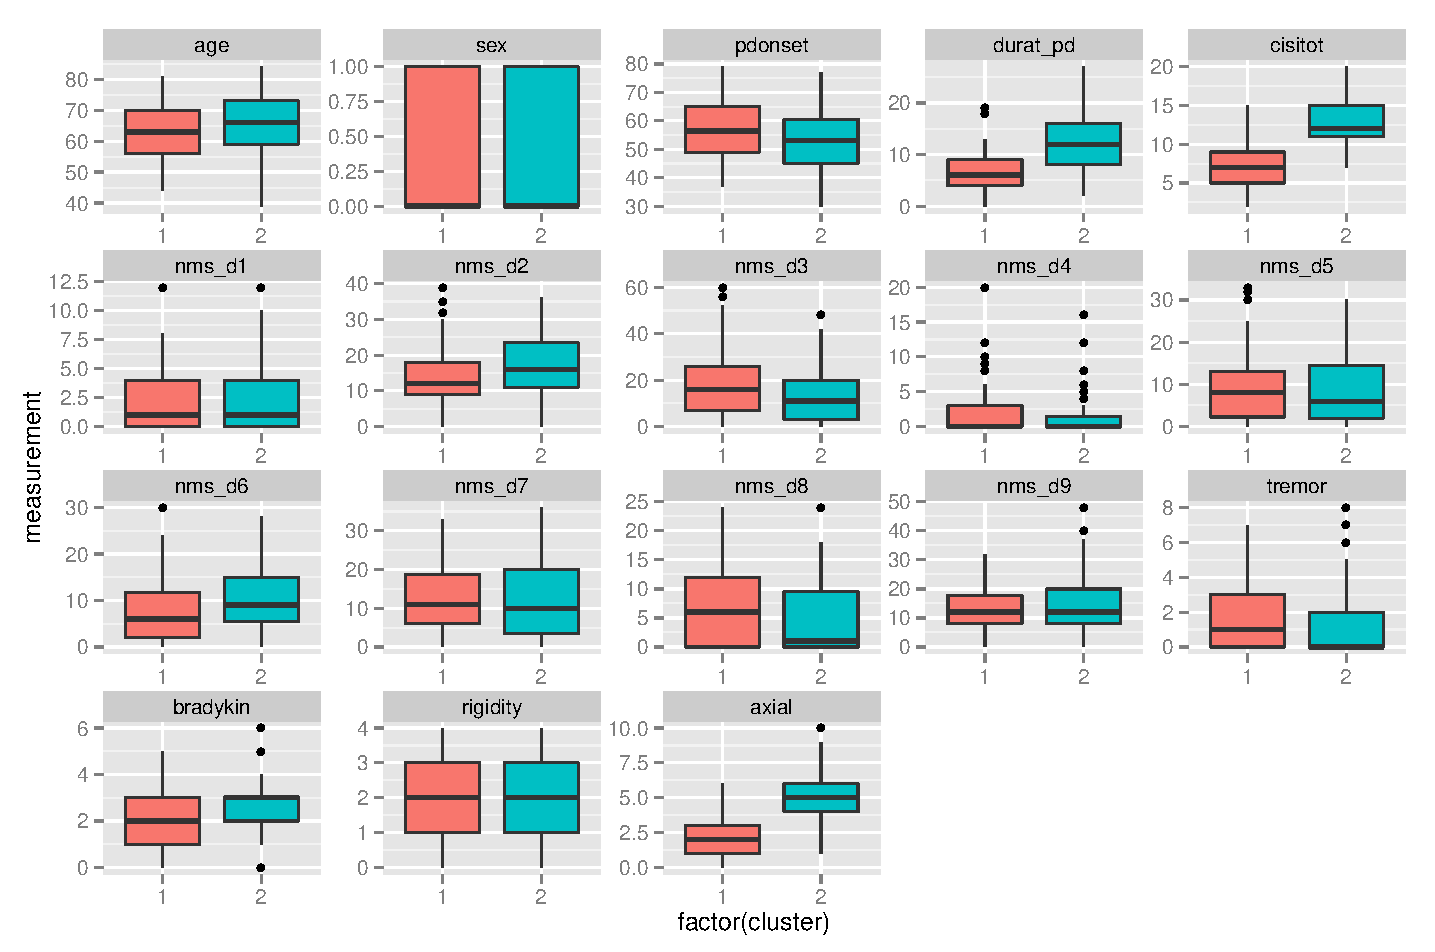
\includegraphics[width=\linewidth]{c1-summaries-2.pdf}
  \caption{Clustering on nonmotor group: $k = 2$}
  \label{fig:c1-summaries-2}
\end{figure}
\begin{figure}[h]
  \centering
  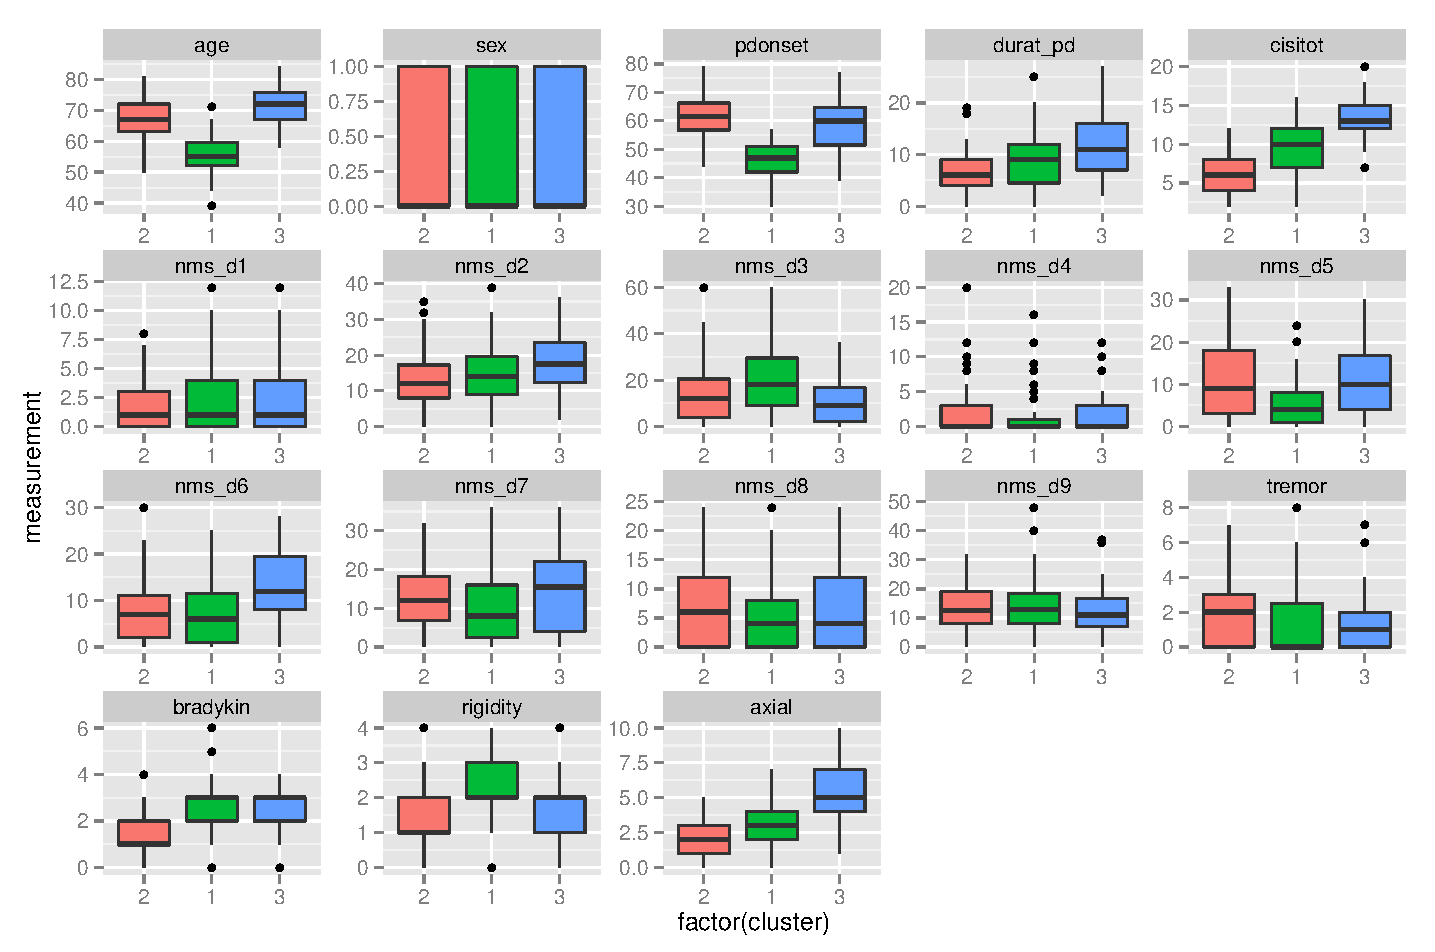
\includegraphics[width=\linewidth]{c1-summaries-3.pdf}
  \caption{Clustering on nonmotor group: $k = 3$}
  \label{fig:c1-summaries-3}
\end{figure}
\begin{figure}[h]
  \centering
  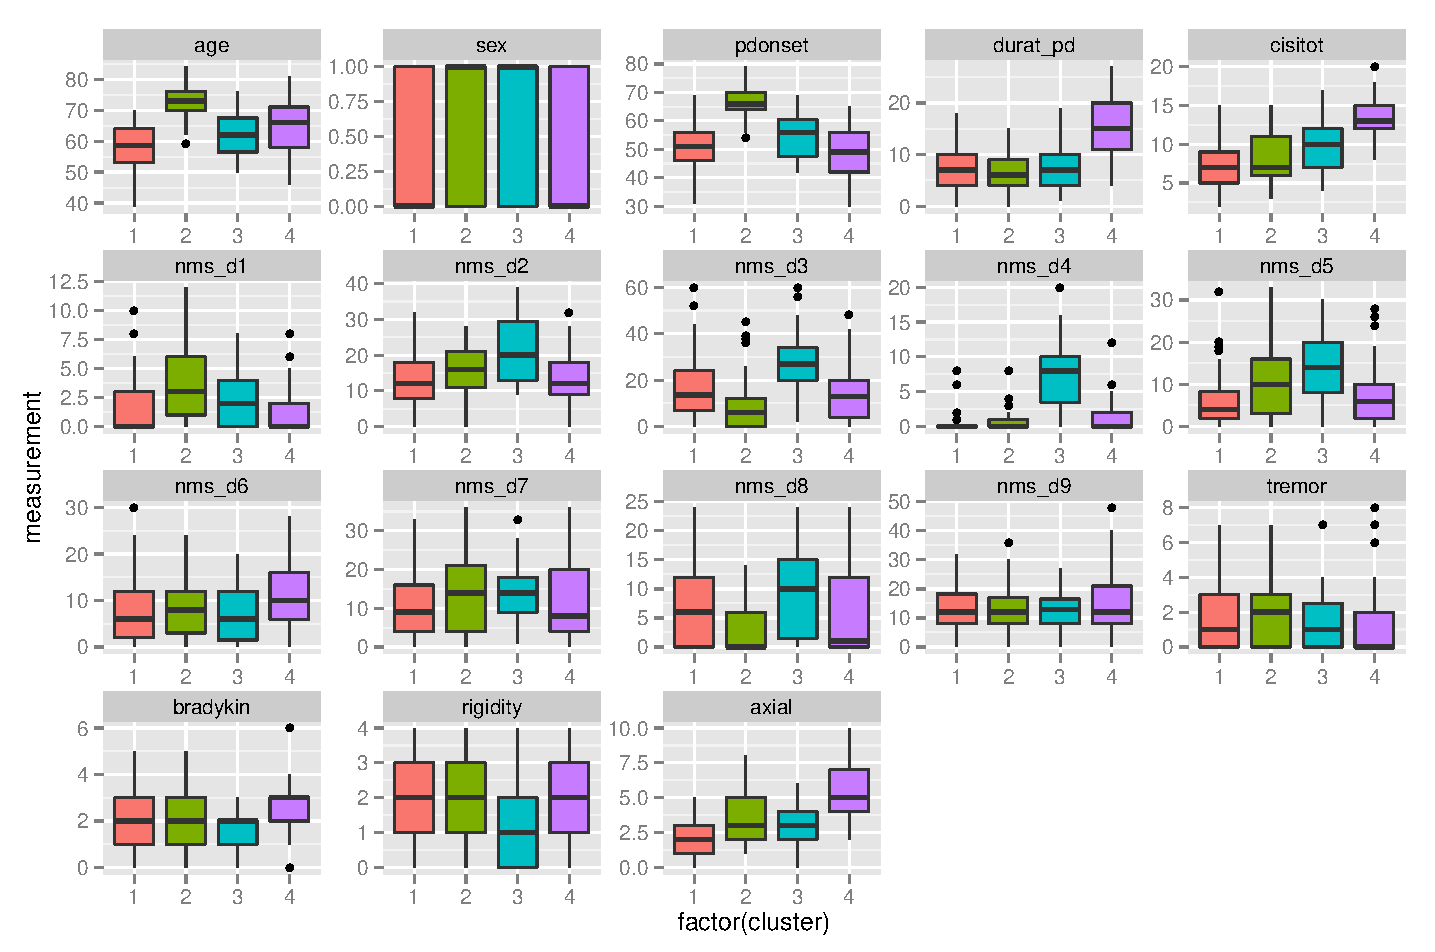
\includegraphics[width=\linewidth]{c1-summaries-4.pdf}
  \caption{Clustering on nonmotor group: $k = 4$}
  \label{fig:c1-summaries-4}
\end{figure}


\section{Modeling}

One further step of this investigation was to produce accurate, practical
models that could be used in a clinical setting to predict the subtype of PD
based on previous clustering results. Cluster assignments were treated as
labels in a supervised classification problem in an attempt to produce useful
models.

\subsection{One-versus-all decision trees}
\label{sub:ova}

While the decision tree in Figure~\ref{fig:kmeans-dtree-4} is useful, it could
be considered overly complicated. Additionally, a model is not necessarily
needed to make simpler diagnoses such as classifying a patient as mildly
affected (subtype 4) or severely affected (subtype 2). One-versus-all (OVA)
decision trees were thus considered, in order to isolate the classification
problem and look at possible distinguishing characteristics of individual
subtypes. These OVA decision trees for all 4 subtypes are located in
Figures~\ref{fig:4va},~\ref{fig:1va},~\ref{fig:3va}, and~\ref{fig:2va}.

\subsubsection{4 (mild)}
This tree is very odd. The root node considers nms\_d9 $< 7.5$ (miscellaneous)
and classifies by far the biggest majority of negative examples when this
symptom is milder, even though the subgroup 4 is the mild subtype. After
intuitively then classifying on the mildness of rigidity the tree then proceeds
to classify once again negative examples based on mildness of nms\_d2 (sleep)
and positive examples solely based on more severe manifestations of nms\_d2,
despite the means of these nonmotor symptoms being quite similar according to
the boxplots.  However, accuracy on the final node is quite poor (61
misclassifications) which could be an indicator that the cluster is not well
defined.

\subsubsection{1 (nonmotor-predominant)}
Quite characteristically, this OVA decision tree clusters first on the severity
of bradykinesia. When mild (i.e.\ $< 2.5$), all of the subsequent decision
nodes ask whether the patient has correspondingly severe forms of primarily
nms\_d3 (mood/cognition), then nms\_d7 (urinary) and nms\_d9 (miscellaneous).

When bradykinesia (and all motor symptoms) are relatively severe, however,
there is still a small subset of patients who classify into subtype 1 by having
severe nms\_d2 (sleep) symptoms. While I am not sure if the sample size is
large enough here (9/34), I propose this could be one of the ``subtypes'' of
the nonmotor-predominant subtype, i.e.\ a group that, when accompanied with
high motor symptoms, generally will have high nonmotor symptoms manifest
primarily in the form of sleep disorders. This aligns with the findings
previously mentioned in Section~\ref{sub:nms-interp} a disjunct between
symptoms nms\_d2 and nms\_d3. As briefly mentioned in that section, axial motor
symptom severity also plays a role. In this tree, mildness of axial symptoms is
the main classifier of 280 negative examples when identifying
nonmotor-predominant
subtypes, indicating it is an important distinguishing factor of this unique
group of 34 nonmotor-predominant PD patients.

More discussion in the
conclusion.

\subsubsection{3 (motor-predominant)}

This tree classifies overwhelmingly on severity of bradykinesia, with 476
negative examples when bradykinesia is less than 2.5. The resulting tree is
quite complex, but generally, nodes check again for severity of motor
symptoms (tremor is the next node) and end up classifying positive examples
based on both mildness of nonmotor symptoms and severity of motor symptoms. For
example, in the furthest right branch, once nms\_d2 (as we know, an important
feature) is established to be relatively mild (< 12), the test for subtype 3
involves two more nodes verifying the severity of rigidty and tremor. Similar
behavior can be found in the tree branch testing nms\_d7 and nms\_d6, then
rigidity and axial.

\subsubsection{2 (severe)}

The OVA tree for severely affected in all areas is predictable, testing
entirely on whether or not symptoms (both motor and nonmotor) are relatively
severe. Ppositive nodes always appear to the right (no) of less-than checks.
Interestingly, however, nms\_d4 (percep/hallucinations), previously not of note, is used twice as the
root node of a tree and again further down. As the boxplot display in
Figure~\ref{fig:kmeans-dtree-4} shows, nms\_d4 is perhaps the most
distinguishing symptom of subtype 4 against nonmotor-predominant subtype 1 in
particular, as subtype 1 is relatively mild, in contrast to relatively
comparable levels of severity for other nonmotor symptoms. This shows that
issues with
perception and hallucinations generally occur in only the most severe cases of
PD, and are relatively rare when a patient exhibits a nonmotor-predominant form
of PD.

\begin{figure}[h]
  \centering
  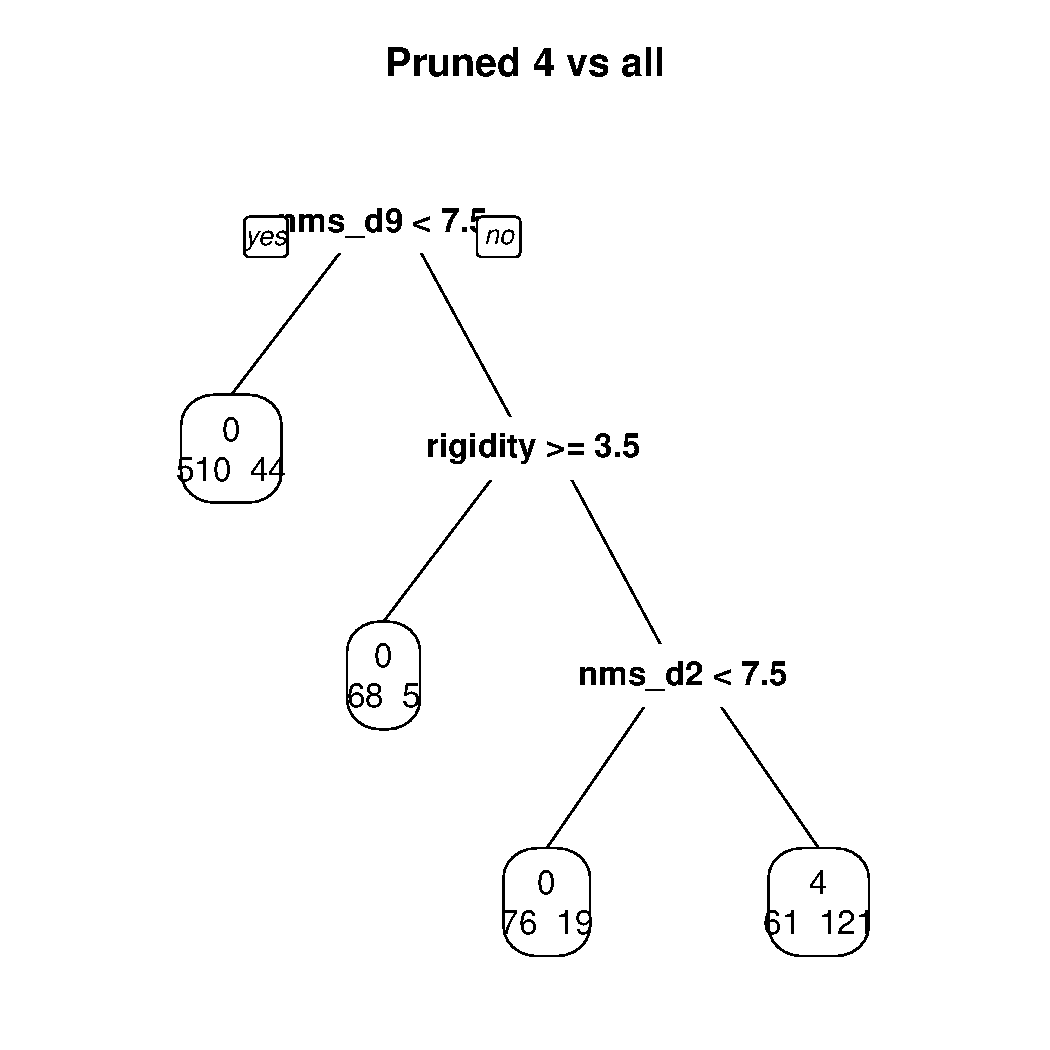
\includegraphics[width=\linewidth]{dtree-4va-pruned.pdf}
  \caption{Cluster 4 (mild) vs all}
  \label{fig:4va}
\end{figure}

\begin{figure}[h]
  \centering
  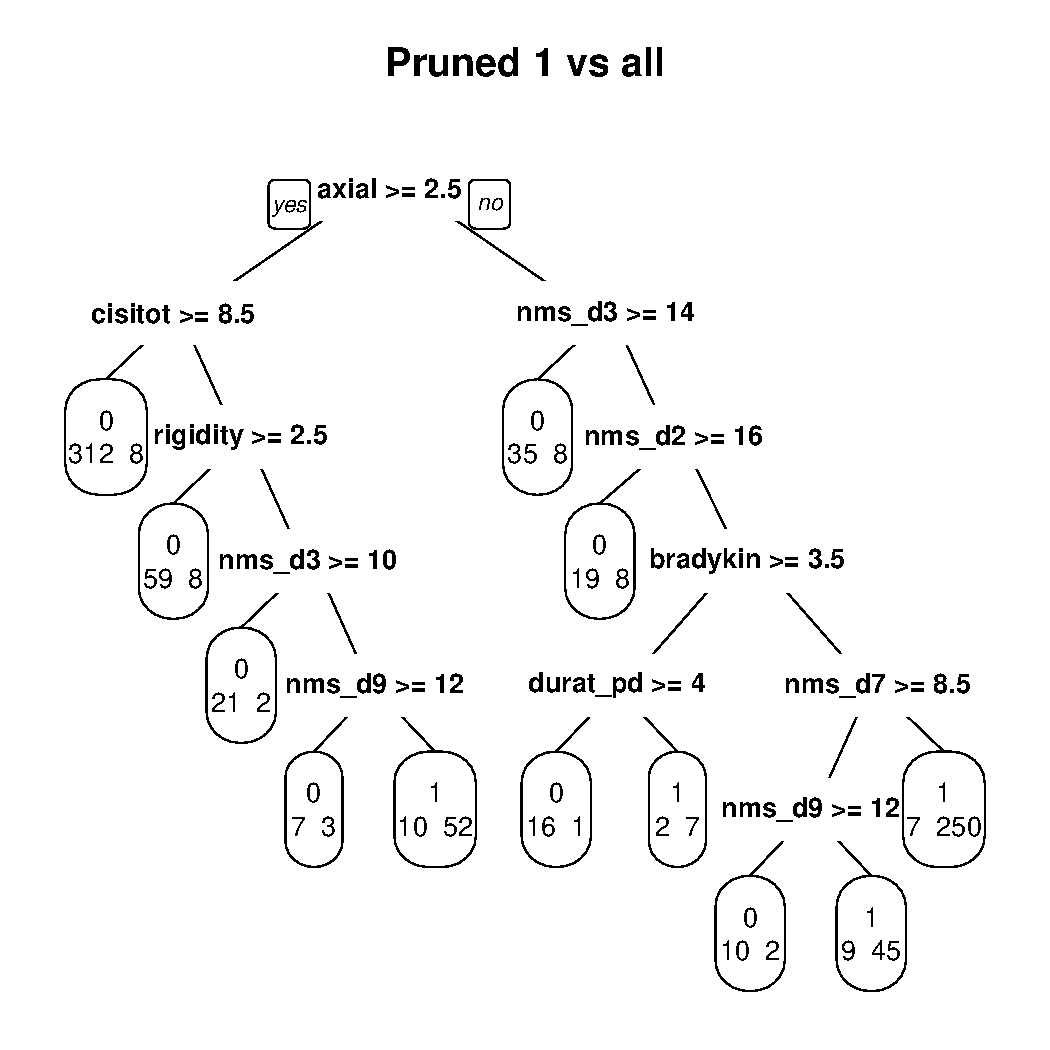
\includegraphics[width=\linewidth]{dtree-1va-pruned.pdf}
  \caption{Cluster 1 (nonmotor-dominated) vs all}
  \label{fig:1va}
\end{figure}

\begin{figure}[h]
  \centering
  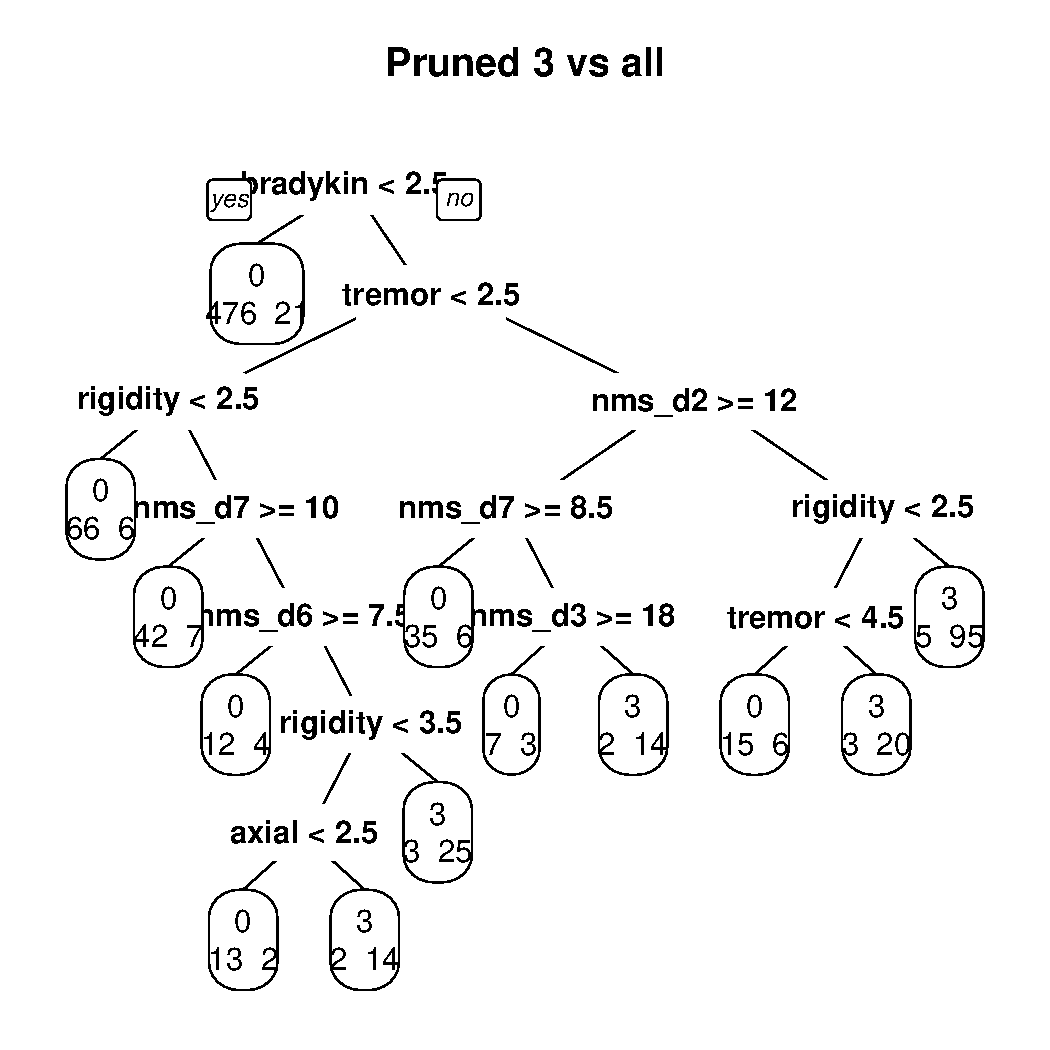
\includegraphics[width=\linewidth]{dtree-3va-pruned.pdf}
  \caption{Cluster 3 (motor-dominated) vs all}
  \label{fig:3va}
\end{figure}

\begin{figure}[h]
  \centering
  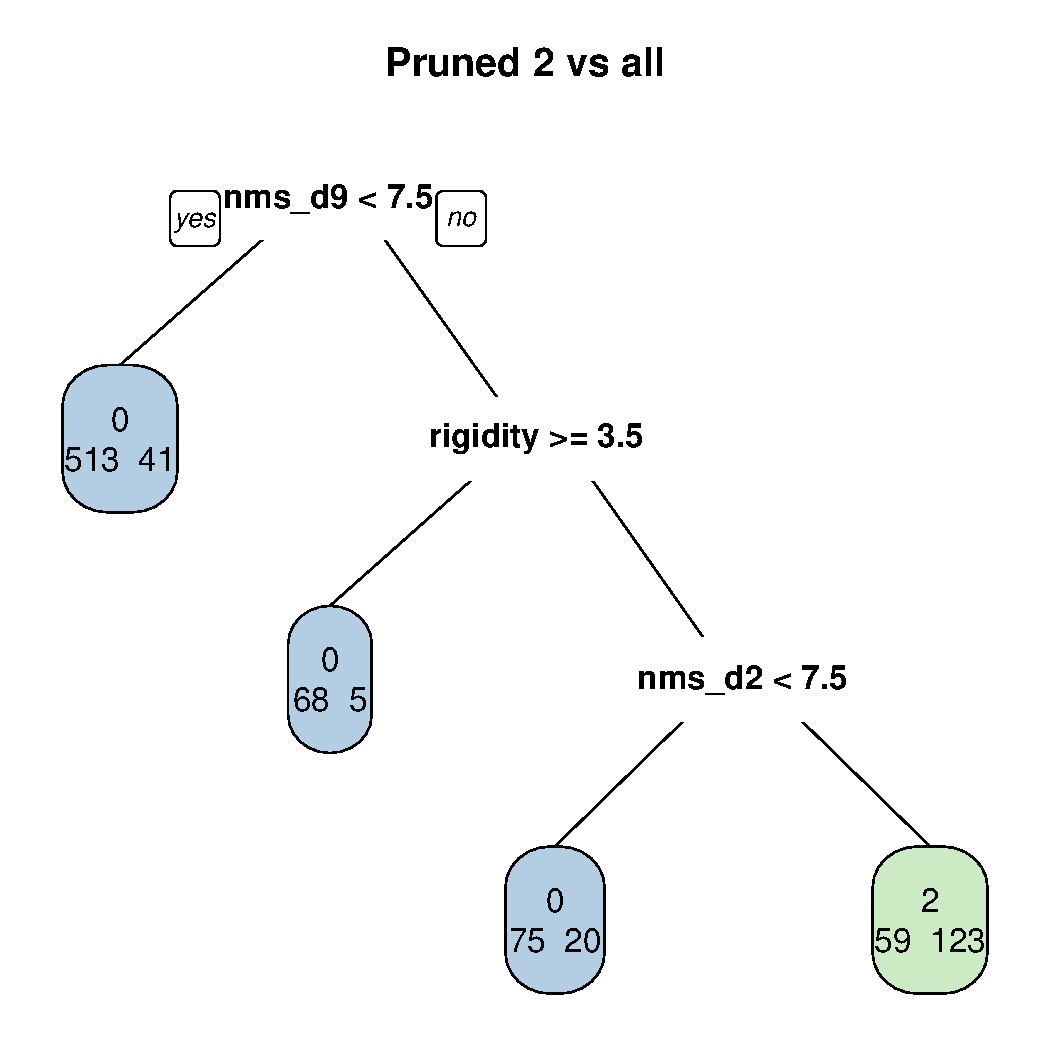
\includegraphics[width=\linewidth]{dtree-2va-pruned.pdf}
  \caption{Cluster 2 (severe) vs all}
  \label{fig:2va}
\end{figure}

\section{Conclusion}

$k$-means clustering on this Parkinsons' Disease data set reveals clusters that
confirm previous computationally-based findings in the field
\cite{vanrooden10}, mainly concerning the identification of four subtypes of
Parkinson's disease: mild, nonmotor-predominant, motor-predominant, and severe.
The most important nonmotor symptoms in determining these clusters were nms\_d2
(sleep) and nms\_d3 (mood/cognition), which echo findings of Fereshtehnejad's
longitudinal study \cite{fereshtehnejad15}. More work

Nonmotor symptoms nms\_d2 and nms\_d3 became critical not only in
classification trees distinguishing between the various symptoms but in the
nonmotor-predominant subgroup itself, where both standard $k$-means analysis
and decision tree branches show two possible trends in the
manifestation of nonmotor-predominant PD:

\begin{itemize}
  \item[1.] Axial and sleep-severe PD
  \item[2.] mood/cognition-severe PD
\end{itemize}

I am, however, not sure if these groups hae enough members to warrant a
subtype, or whether this could just be chance or noise.

It remains to be seen whether these classification models, especially the
one-vs-all decision trees, are useful in clinical practice.

\subsection{Bayesian Networks}

\subsubsection{On all data}

I decided to discretize the data into three uniform-width groups based on the
scales of each symptom. In other words, each symptom was discretized into a
mild, moderate, and severe bin. Continuous data was unreliable on my computer,
and updating intricately connected nodes like nms\_d2 resulted in slowdowns and
crashes on my computer.

Two bayesian network algorithms were tried: the default Bayesian score-search
algorithm and the PC conditional independence tests algorithm. I couldn't find
the exact name of the Bayesian search implementation, but it was the default
method used by GeNIe. GeNIe files will be attached electronically.

I assume these models are to be looked at by Dr. Mart\'in. I have not done too
much investigation myself, as I'm not exactly sure what I'm looking for).

\subsubsection{On nms-dominated data}
I tried to construct Bayesian networks based on the nms-dominated subtype, but
the data was too sparse to create a very informative network, even when leaving
the information continuous. However, I'm not sure this is necessary. If it is,
I can work on this problem more.

\begin{thebibliography}{9}

\bibitem{fereshtehnejad15}
Fereshtehnejad et al (June 15, 2015). New Clinical Subtypes of Parkinson
Disease and Their Longitudinal Progression

\bibitem{vanrooden10}
van Rooden et al (2010). The Identification of Parkinson's Disease Subtypes
Using Cluster Analysis: A Systematic Review

\end{thebibliography}

\end{document}
